\section{Experimentování}
Cílem experimentování je zjistit, jak se CA chová a jestli splňuje některé
z předpokladů, pokud nějaké jsou.

Pro přehlednost jsou pravidla rozdělená barvy (každému pravidlu
v rozmezí 0 až 255 je přiřazena jiná barva), aby bylo zjevné, kdy dojde
k aplikaci jiného pravidla.
Černá barva znázorňuje stav 1 buňky 1. generace, bílá barva značí stav 0 buňky,
ostatní barvy značí stav 1 buňky.

\begin{figure}[h]
	\centering
	\frame{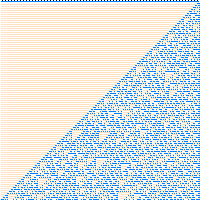
\includegraphics[width=0.75\textwidth]{rule_30_45.png}}
	\caption{200 generací pravidla 30 a 45 (střídající se), počáteční stav (0, 0, 1, 0, 0, 1, ...)}
\end{figure}

\newpage
\subsection{Aplikování pseudo-náhodného pravidla}
Aplikováním pseudo-náhodného (dále jen náhodného) pravidla rozumíme to,
že pro každou generaci bude aplikováno jiné náhodně vygenerované pravidlo.
Předpokladem pro chování tohoto CA bylo, že bude vykazovat náhodné
chování alespoň v některých případech.
Výsledek experimentu však ukázal opak - ve většině případů byl výsledek téměř stejný
a ten je, že po pár generacích se pouze střídají generace, kdy jsou všechny buňky
ve stavu 0 s generací, kdy jsou všechny buňky ve stavu 1.

Aplikace náhodného pravidla, 100 generací, počáteční stav (0, 0, 1, 0, 0, 1, ...):
\begin{figure}[h]
	\centering
	\frame{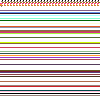
\includegraphics[width=0.35\textwidth]{rule_random_1.png}}
	\hspace{3em}
	\frame{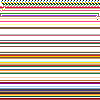
\includegraphics[width=0.35\textwidth]{rule_random_2.png}}
	\caption{Výsledný vzor pro většinu případů.}
\end{figure}

\begin{figure}[h]
	\centering
	\frame{
\includegraphics[width=0.35\textwidth]{rule_random_0.png}}
	\hspace{3em}
	\frame{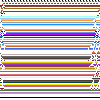
\includegraphics[width=0.35\textwidth]{rule_random_3.png}}
	\caption{V minimálním množství případů po několik generací
	vykazovaly CA chování, jehož výsledný vzor můžeme přirovnat k růstu kořenů.
	Nakonec ale vždy konvergují do stejného stavu.}
\end{figure}

Při zvolení náhodného pravidla je totiž velká šance, že buňky nepřežijí po
dostatečné množství generací - v určitý moment dojde k tomu, že všechny buňky v
dané generaci budou mít stejný stav a jediné pravidlo, které tento stav změní,
je pravidlo, které je všechny nastaví do opačného stavu.

\newpage
\subsection{Aplikace 2 pravidel}
Předpoklad pro chování tohoto CA není jednoduché určit.
Bylo předpokládáno, že nejspíše dojde k tomu, že výsledný vzor
bude připomínat kombinace jevů těchto vzorů
- pokud jeden vzor vytváří diagonální čáry a druhý trojúhelníky,
tak jejich kombinace bude vytvářet trojúhelníky s menším náklonem.

Tento předpoklad v některých případech platil:
\begin{figure}[h]
	\centering
	\frame{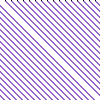
\includegraphics[width=0.35\textwidth]{rule_14.png}}
	\hspace{3em}
	\frame{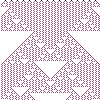
\includegraphics[width=0.35\textwidth]{rule_18.png}}
	\caption{Pravidla 14 a 18 s počátečním stavem (0, 0, 0, 0, 0, 1, ...).}
\end{figure}

\begin{figure}[h]
	\centering
	\frame{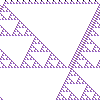
\includegraphics[width=0.35\textwidth]{rule_14_18.png}}
	\caption{Kombinace pravidel 14 a 18 se stejným počátečním stavem;
	pravidla se periodicky střídají}
\end{figure}


\newpage
V jiných případech předpoklad neplatil:
\begin{figure}[h]
	\centering
	\frame{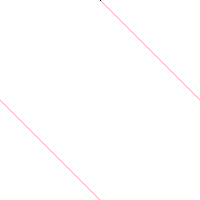
\includegraphics[width=0.3\textwidth]{rule_10.png}}
	\hspace{3em}
	\frame{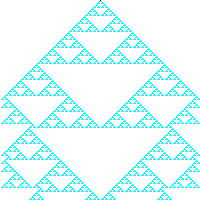
\includegraphics[width=0.3\textwidth]{rule_22.png}}
	\caption{Pravidla 10 a 22}
\end{figure}

\begin{figure}[h]
	\centering
	\frame{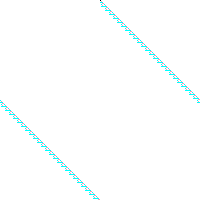
\includegraphics[width=0.3\textwidth]{rule_10_22_ring.png}}
	\caption{Kombinace pravidel 10 a 22; pravidla se periodicky střídají}
\end{figure}

\begin{figure}[h]
	\centering
	\frame{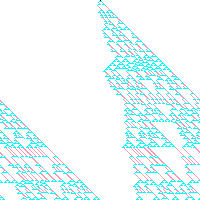
\includegraphics[width=0.3\textwidth]{rule_10_22_rand.png}}
	\caption{Kombinace pravidel 10 a 22; pravidla se náhodně střídají}
\end{figure}

\subsection{Aplikace 3 a více pravidel a zajímavé útvary}
Pro aplikaci více pravidel nebyl již určen žádný předpoklad pro chování takového CA.
Cílem tohoto experimentu je dosáhnout nalezení zajímavých útvarů, které je možné
získat kombinací více pravidel.

Na obrázcích níže je možné vidět některé zajímavé útvary nalezené kombinací pravidel.
U popisu obrázků je napsané, které pravidla jsou aplikována.
Všechny pravidla se periodicky střídají.

\begin{center}
	\begin{minipage}{0.32\linewidth}
		\frame{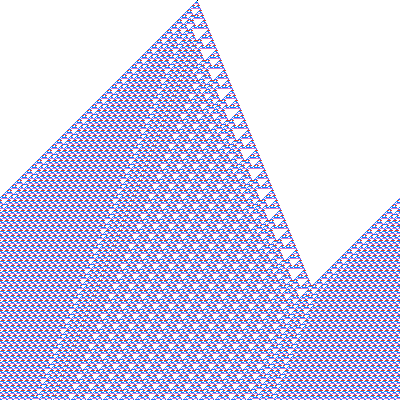
\includegraphics[width=\linewidth]{rule_208_30_250_60_126.png}}
		\captionof{figure}{(208, 30, 250, 60, 126)}
	\end{minipage}
	\hfill
	\begin{minipage}{0.32\linewidth}
		\frame{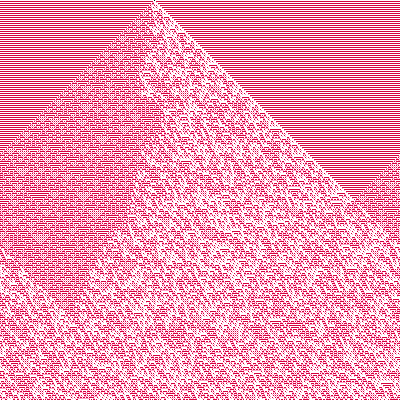
\includegraphics[width=\linewidth]{rule_105_106.png}}
		\captionof{figure}{(105, 106)}
	\end{minipage}
	\hfill
	\begin{minipage}{0.32\linewidth}
		\frame{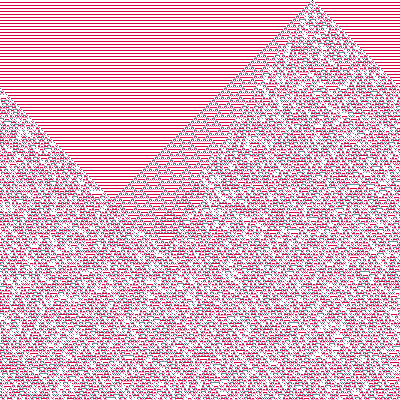
\includegraphics[width=\linewidth]{rule_89_105_106.png}}
		\captionof{figure}{(89, 105, 106)}
	\end{minipage}%
\end{center}

\begin{center}
	\begin{minipage}{0.32\linewidth}
		\frame{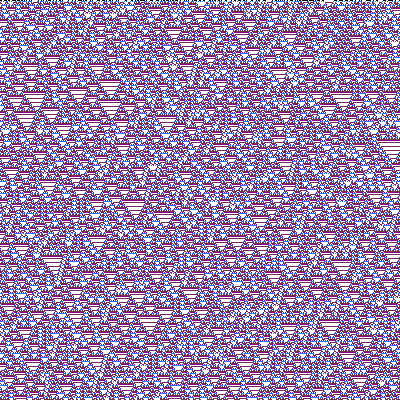
\includegraphics[width=\linewidth]{rule_60_89_110_178.png}}
		\captionof{figure}{(60, 89, 110, 178)}
	\end{minipage}
	\hfill
	\begin{minipage}{0.32\linewidth}
		\frame{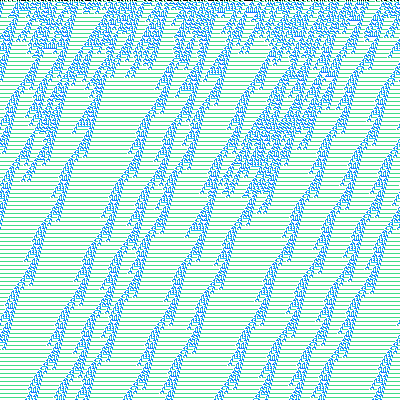
\includegraphics[width=\linewidth]{rule_15_22_30_60.png}}
		\captionof{figure}{(15, 22, 30, 60)}
	\end{minipage}
	\hfill
	\begin{minipage}{0.32\linewidth}
		\frame{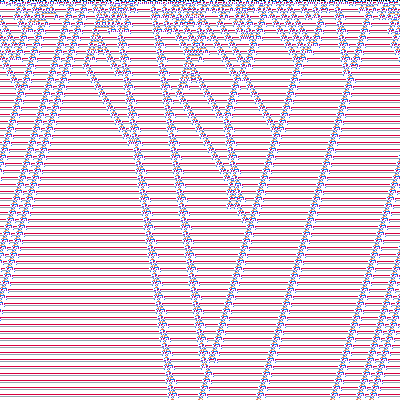
\includegraphics[width=\linewidth]{rule_30_105_69_91_60_232_86.png}}
		\captionof{figure}{(30, 105, 69, 91, 60, 232, 86)}
	\end{minipage}%
\end{center}

\begin{center}
	\begin{minipage}{0.32\linewidth}
		\frame{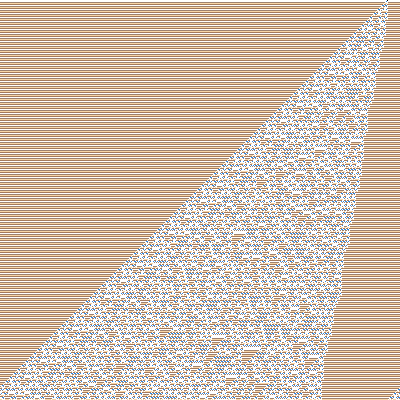
\includegraphics[width=\linewidth]{rule_56_41_195_244.png}}
		\captionof{figure}{(64, 41, 195, 244)}
	\end{minipage}
	\hfill
	\begin{minipage}{0.32\linewidth}
		\frame{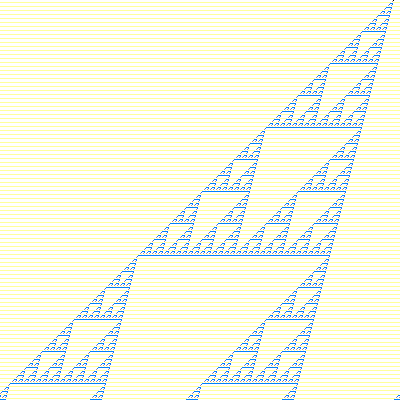
\includegraphics[width=\linewidth]{rule_16_90_30_60.png}}
		\captionof{figure}{(16, 90, 30, 60)}
	\end{minipage}
	\hfill
	\begin{minipage}{0.32\linewidth}
		\frame{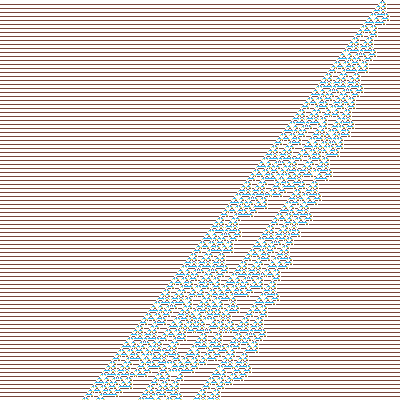
\includegraphics[width=\linewidth]{rule_18222673.png}}
		\captionof{figure}{(18, 22, 26, 73)}
	\end{minipage}%
\end{center}
